%%%%%%%%%%%%%%%%%%%%%%%%%%%%%%%%%%%%%%%%%%%%%%%%%%%%%%%%%%%%%%%%%%%%%%%%%%%%%%%
%%%%%%%%%%%%%%%%%%%%%%%%%%%%%%%%%%%%%%%%%%%%%%%%%%%%%%%%%%%%%%%%%%%%%%%%%%%%%%%
% APPENDIX
%%%%%%%%%%%%%%%%%%%%%%%%%%%%%%%%%%%%%%%%%%%%%%%%%%%%%%%%%%%%%%%%%%%%%%%%%%%%%%%
%%%%%%%%%%%%%%%%%%%%%%%%%%%%%%%%%%%%%%%%%%%%%%%%%%%%%%%%%%%%%%%%%%%%%%%%%%%%%%%
\newpage
\appendix
\onecolumn

\definecolor{darkbrown}{HTML}{8B4513}
\definecolor{navyblue}{HTML}{000080}
\definecolor{darkgreen}{HTML}{008000}
\definecolor{purple}{HTML}{800080}
\definecolor{red}{HTML}{FF0000}

\section{Additional Related Work}

\subsection{Neural Solvers}
Recently, much effort has been made to develop end-to-end neural solvers, especially for combinatorial optimization~\cite{bengio2021machine}. A pointer network as a neural solver was proposed to construct solutions autoregressively in~\citet{vinyals2015pointer}. Some improvements to this work have been made including using an efficient reinforcement learning framework to replace the original supervised learning~\cite{bello2016neural} and adopting an attention model to replace the pointer network~\cite{kool2018attention,deudon2018learning}. Among these variants~\cite{xin2020step,kwon2020pomo,kwon2021matrix}, a multiple optimal policy proposed in~\cite{kwon2020pomo} archives the state-of-the-art performance on diverse problems of small or moderate sizes. Recent progress, leveraging a heavy encoder and light decoder, enhances its scalarization~\cite{drakulic2023bq,luo2023neural}.

 
Some effort has also been made to hybridize neural solvers and classic heuristic algorithms including heat map-based methods~\cite{joshi2019efficient,fu2021generalize, qiu2022DIMES}, heat map guided beam search~\citep{joshi2019efficient}, Monte Carlo tree search (MCTS)~\cite{fu2021generalize}, dynamic programming~\cite{kool2022deep}, and guided local search~\cite{hudson2021graph,sui2023neuralgls}. 
The hybridization often requires significant effort to design and train domain neural models.



\subsection{Prompt Engineering}
LLMs with simple promoting face challenges in solving complex reasoning tasks~\cite{chu2023survey}. To address this challenge, Chain-of-Thought (CoT)~\cite{wei2022chain} was proposed to do in-context learning with step-by-step reasoning processes to enhance the reasoning ability of LLMs without human annotation. 

Consequently, there have been many extensions and modifications on CoT such as multi-sampling, tree-of-thoughts~\cite{long2023large}, graph-of-thoughts~\cite{yao2023beyond}, algorithm-of-thoughts~\cite{sel2023algorithm}, and automatic CoT construction~\cite{kojima2022large,xu2023reprompting}. The prompt strategies used in EoH can be regarded as variants of CoT for the design of heuristics with parent heuristics and instructions as in-context information. 

% \section{More Ablation Studies}

% \paragraph{Search Methods} 
% EoH uses an evolutionary algorithm as its search engine for exploring the space of heuristics. In the following, we investigate if other search methods are used to replace evolutionary algorithms in EoH. We consider the following three search methods: 
% \begin{itemize}
%     \item Local Search (LS):  LS maintains a single solution (a heuristic in our work) at each iteration and explores a neighborhood of its current to find a better solution.  
    
%     \item Simulated Annealing (SA): It also maintains a single solution at each iteration. It samples a solution from a neighborhood of the current solution. If this sampled solution is better than the current solution, it will replace the current solution. If it is worse,  SA still does replacement with some probability. 
    
%     \item Random sampling: it simply generates new heuristics by requesting LLMs with the initialization prompt.
% \end{itemize}
% In our experiments, the computational budget for EoH with each method is the same (2,000 requests to LLMs). The results are summarized in the following table. Results show that evolutionary algorithms (EAs) clearly outperform other search methods in EoH. It indicates that population search is very useful in EoH. Single-point-based search methods (LS and SA) vary across different runs.



% \begin{table}[htbp]
% \centering
% \caption{Comparison of different search methods: Average gap (\%) to LB on bin packing instances (The smaller the better)}
% \resizebox{0.48\textwidth}{!}{%
% \begin{tabular}{lllllll}
% \toprule
% Method  & Run 1 & Run 2 & Run 3 & Average & Deviation \\
% \midrule
% Sampling     & 2.76  & 1.92  & 2.65  & 2.44   & 0.82      \\
% LS            & 2.61 & 0.95 & 1.15 & 1.58    & 0.74      \\
% SA            & 0.67 & 0.74 & 1.56  & 0.99    & 0.40      \\
% % EoH          & 0.75 & 0.91 & 0.72 & 0.80    & 0.08      \\
% % EoH         & 0.70 & 0.61 & 0.60 & 0.64    & 0.04      \\
% EoH        & 0.68 & 0.67 & 0.62 & 0.66    & 0.03     \\
% \bottomrule
% \end{tabular}%
% }
% \end{table}



% \paragraph{LLMs} 
% We compare four commonly used LLMs: GPT3.5, Gemini Pro, CodeLlama, and Deepseek. All experiments are carried out using the same experimental settings three times on the online bin packing problem. In general, EoH can generate good-performance heuristics using these different LLMs. EoH using different LLMs with 2,000 requests to LLMs performs better than randomly requesting GPT3.5 10,000 times. Nevertheless,  our experimental results also show that GPT3.5 and Gemini Pro outperforms other LLMs. 
% %This could be attributed to the EoH's demands on both language comprehension and code generation, posing difficulties for smaller or domain-specific LLMs.

% \begin{table}[htbp]
% \centering
% \caption{Comparison of EoH with different LLMs: Average gap (\%) to LB on online bin packing problem (The smaller the better)}
% \resizebox{0.48\textwidth}{!}{%
% \begin{tabular}{llllll}
% \toprule
% Method & LLM           & Run 1 & Run 2 & Run 3 & Average \\
% \midrule
% Sampling      & GPT3.5  & 2.76  & 1.92  & 2.65  & 2.44  \\
% EoH    & CodeLlama & 0.93  & 0.62  & 1.66  & 1.07        \\
% EoH    & Deepseek      & 1.01  & 1.47  & 1.75  & 1.41       \\
% EoH    & Gemini Pro    & 0.92  & 0.61  & 0.61  & 0.71         \\
% EoH    & GPT3.5        & 0.68  & 0.67  & 0.62  & 0.66       \\
% \bottomrule
% \end{tabular}%
% }
% \end{table}
    
% \paragraph{ Use of Expert Heuristics}
% We investigate the impact of the use of existing heuristics (expert heuristics) in EoH. Take the bin packing problem as an example, we adopt the heuristic provided in FunSearch paper~\cite{romera2023mathematical} as the existing expert heuristic and put it into the initial population of EoH. The rest of the initial individuals are randomly generated. The results are given in Table~\ref{fig:expert}. We term the EoH with an expert in the initial population as EoH expert and compare it to the original EoH and FunSearch. The results show that the adoption of elite expert heuristic benefits in the population benefits the final results in our test case. The EoH expert clearly surpasses both FunSearch and EoH. The knowledge of expert heuristics can be inherited and evolved during evolution to produce better heuristics. 

% \begin{table}[htbp]
% \centering
% \caption{EoH with an existing expert heuristic.}~\label{fig:expert}
% \resizebox{0.4\textwidth}{!}{%
% \begin{tabular}{lllll}
% \toprule
% Method     & Run 1 & Run 2 & Run 3 & Average \\
% \midrule
% FunSearch  & 0.94  & 0.82  & 1.15  & 0.97    \\
% EoH        & 0.68  & 0.67  & 0.62  & 0.66    \\
% EoH expert & 0.57  & 0.55  & 0.52  & 0.55   \\
% \bottomrule
% \end{tabular}
% }
% \end{table}


\section{Online Bin Packing Problem}

\subsection{Prompt Engineering}
In the following, we introduce the detailed prompt engineering used for online bin packing problem. The prompt engineering for each evolution procedure consists of five main parts: 1) Task description, 2) Strategy-specific prompt, 3) Expected output, 4) Note, and  5) Parent heuristic(s). Figure~\ref{fig:prompt_bp} presents two examples of prompts: initialization prompt and E2 prompt. The prompt engineering for other operators (E1, M1, M2, and S1) has the same structure as these two examples and is not listed for brevity. The five parts in different colors are introduced as follows:

\begin{itemize}[itemsep=-3pt]
    \item \textcolor {darkbrown}{\textbf{Task description}}: It informs LLMs of the problem description. Different prompt strategies usually share the same task description.
    \item {\textbf{Strategy-specific prompt}}: It instructs LLMs to do reasoning over the in-context information and generate new heuristics as well as its corresponding code implementation. Different prompt strategies have different strategy-specific prompts. For example, during initialization, we instruct the LLM to create a totally new heuristic. During evolution, we request LLM to perform different types of reasoning over parent heuristic(s) to explore the heuristic search space.
    \item \textcolor{navyblue}{\textbf{Expected output}}: It asks the LLM to provide a description of the designed heuristic and then produce the code implementation for the heuristic. In this paper, the code implementation is a function in Python. We explicitly define the name, input, and output of the code for easy identification by \ourmethod{} framework. 
    \item \textcolor{purple}{\textbf{Note}}: It provides additional instructions for LLM to improve the efficiency and robustness. For example, we may suggest specific types of inputs and outputs and discourage extra explanations to prevent a long response.
    \item \textcolor{darkgreen}{\textbf{Parent heuristic(s)}}: It includes parent heuristic(s) to enable in-context learning over both the linguistic heuristic description and the code implementation. The initialization prompt does not include this part.
\end{itemize}


\begin{figure}
    \centering
    \caption{Two examples of prompt engineering used in initialization prompt and E2 prompt for online bin packing.}
    \label{fig:prompt_bp}

\begin{minipage}{0.38\textwidth}
\small
\begin{dialogbox}
  \textbf{Prompt for Initialization} \\
  
  \textcolor {darkbrown}{ I need help designing a new heuristic that scores a set of bins to assign an item. In each step, the item will be assigned to the bin with the maximum score. If the rest capacity of a bin equals the maximum capacity, it will not be used. The final goal is to minimize the number of used bins.} \\

  Please design a new heuristic.
  
  \textbf{Firstly,} describe your \textcolor{navyblue}{new heuristic and main steps in one sentence}. \\
  \textbf{Next,} implement it in Python as a function named \textcolor{navyblue}{'score'}. This function should accept \textcolor{navyblue}{two inputs: 'item' and 'bins'}. The function should return \textcolor{navyblue}{one output: 'scores'}. \textcolor{navyblue}{'item' and 'bins' are the size of the current item and the rest capacities of feasible bins, which are larger than the item size. The output named 'scores' is the scores for the bins for assignment.}  \\

  \textcolor{purple}{Note that 'item' is of type int, 'bins' is a Numpy array that includes integer values, and 'scores' should be a Numpy array. Avoid utilizing the random component, and it is crucial to maintain self-consistency. Do not give additional explanations.}
\end{dialogbox}
\end{minipage}
\begin{minipage}{0.6\textwidth}
\small
\begin{dialogbox}
  \textbf{Prompt for E2} \\
  
  \textcolor[HTML]{8B4513}{ I need help designing a new heuristic that scores a set of bins to assign an item. In each step, the item will be assigned to the bin with the maximum score. If the rest capacity of a bin equals the maximum capacity, it will not be used. The final goal is to minimize the number of used bins.} \\

  \textcolor{darkgreen}{I have five existing heuristics with their codes as follows: \\
  No.1 Heuristic description: \\
       Code:   \\
       ... \\
  No.5 Heuristic description: \\
       Code: \\  } 
       
   Please help me design a new heuristic that is different from the given ones but can be motivated by them. \\
   \textbf{Firstly,} identify the common idea in the provided heuristics.   \\
   \textbf{Secondly,} based on the backbone idea \textcolor{navyblue}{describe your new heuristic in one sentence.} \\
   \textbf{Thirdly,} implement it in Python as a function named \textcolor{navyblue}{'score'}. This function should accept \textcolor{navyblue}{two inputs: 'item' and 'bins'}. The function should return \textcolor{navyblue}{one output: 'scores'}. \textcolor{navyblue}{'item' and 'bins' are the size of the current item and the rest capacities of feasible bins, which are larger than the item size. The output named 'scores' is the scores for the bins for assignment.}  \\

  \textcolor{purple}{Note that 'item' is of type int, 'bins' is a Numpy array that includes integer values, and 'scores' should be a Numpy array. Avoid utilizing the random component, and it is crucial to maintain self-consistency. Do not give additional explanations.}
\end{dialogbox}
\end{minipage}
\end{figure}


\begin{figure}[htbp]
    \centering
    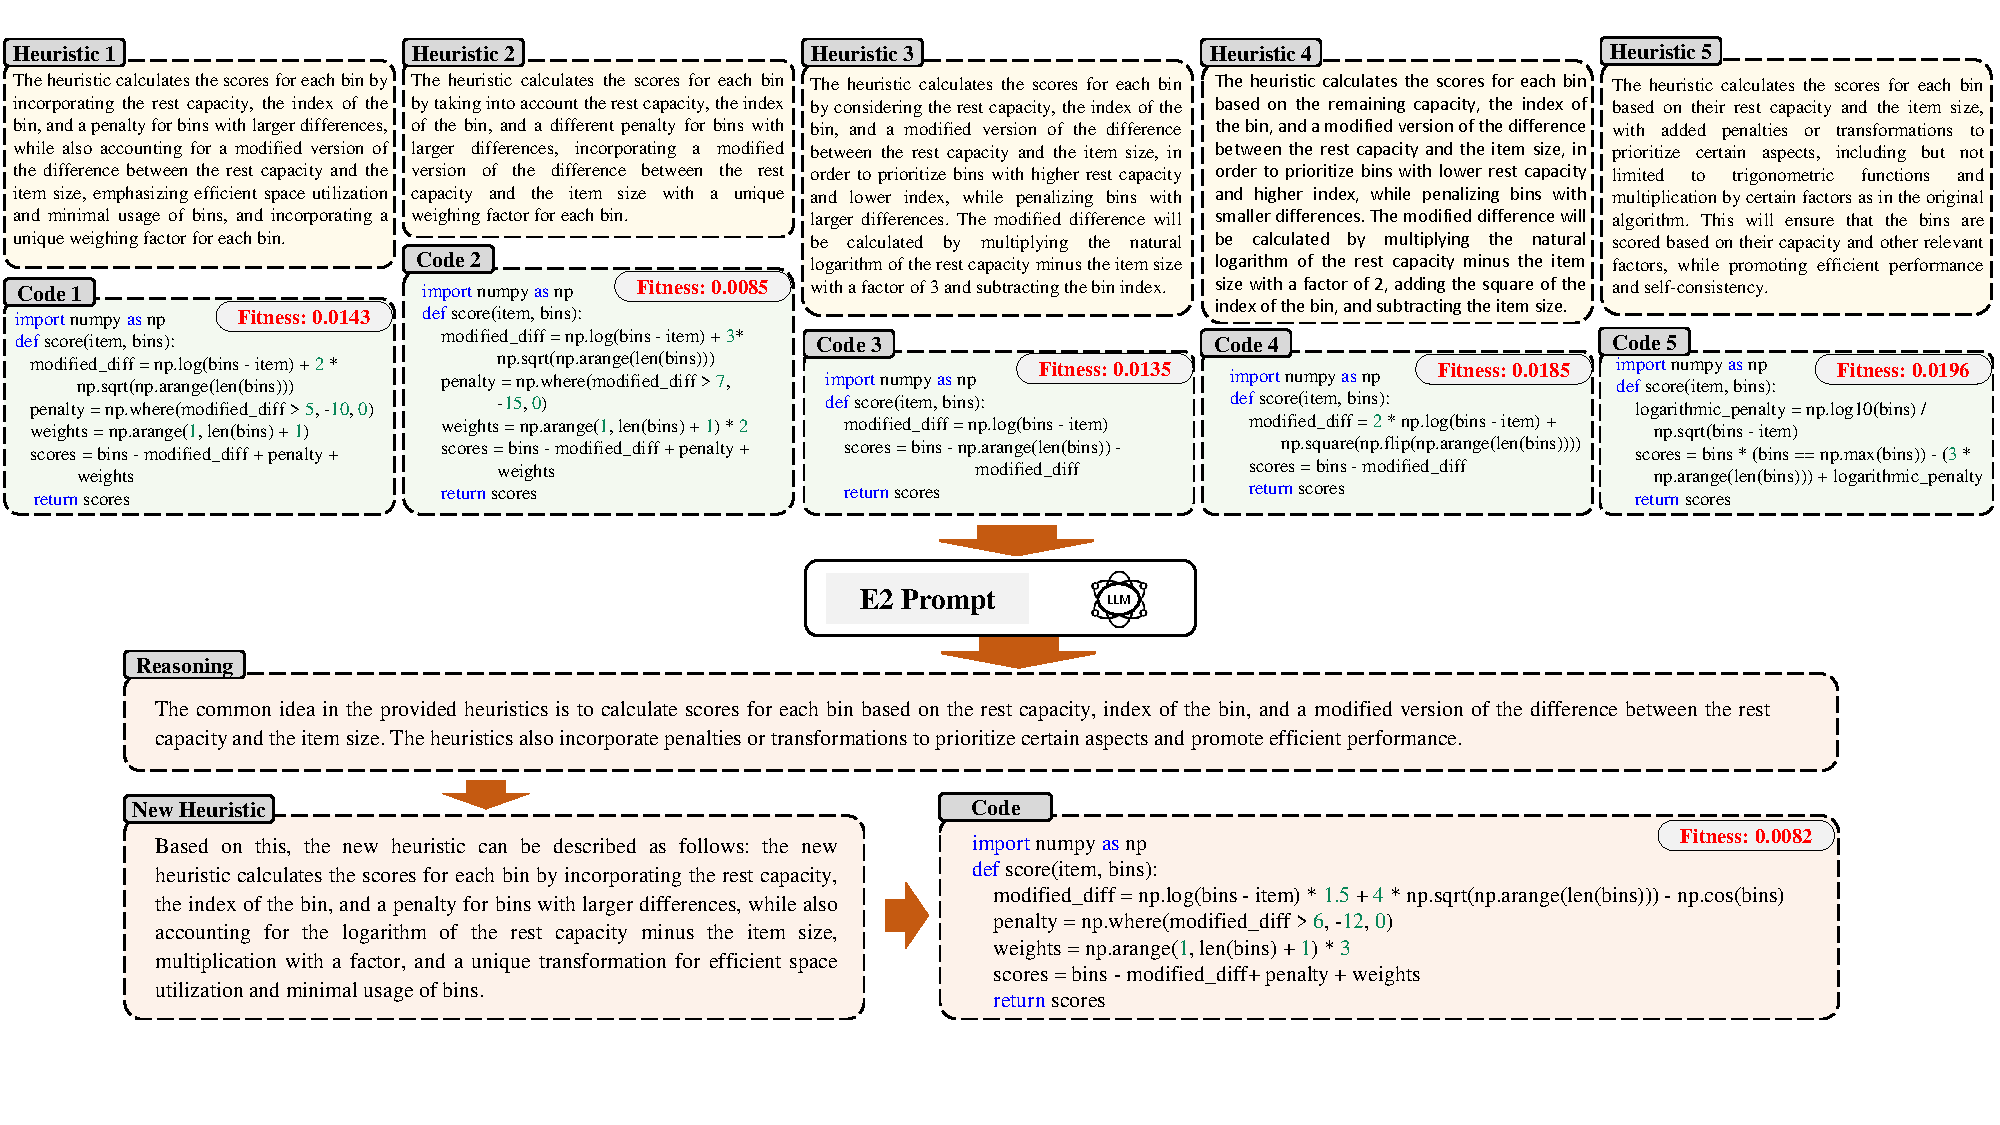
\includegraphics[width=\textwidth]{figures/Fig_E2.pdf}~\label{fig:ee2}
    \caption{Illustration of the generation of new heuristic and its code implementation using E2 prompt in one step in \ourmethod{} on online bin packing problem. Five parent heuristics are selected from the population. E2 prompts LLM to first observe and summarize the common idea in the five heuristics, then design a new heuristic using this idea, and finally give a code implementation for the designed heuristic.}
    \label{fig:enter-label}
\end{figure}


\subsection{Heuristic Evolution}~\label{e2}

% The convergence process of evolution has been introduced in the main paper. We present the detailed process of one step of E2  during the evolution in Figure~\ref{fig:e2}. Five heuristics are selected from the population. Each of them consists of a high-level description of the heuristic and a detailed implementation of Python. These heuristics are fed into the prompt engineering for E2 (introduced in last section) to prompt LLMs. The LLMs are instructed to perform three steps: firstly, identify the common idea in the provided heuristics based on their descriptions and codes. Secondly, design a new heuristic based on its analyse. Thirdly, implement the heuristic in Python with a given name, input, and output. A better heuristic is designed with the identified common idea and the integration of a new logarithm term.

The convergence process of evolution has been discussed in the main part. Figure 6 presents a detailed illustration of  E2 in one generation. Five heuristics are chosen from the population, each of them consists of a high-level description and a detailed Python implementation. These heuristics are then used as inputs for prompt engineering in E2, which was introduced in the previous section. The LLMs are given three instructions: firstly, to identify the shared concept among the provided heuristics based on their descriptions and codes; secondly, to design a new heuristic based on this analysis; and thirdly, to implement the heuristic in Python with a given name, input, and output. The improved heuristic follows the identified common idea and integrates new components.


\subsection{Designed Heuristic}
Comparison of heuristics designed by humans, EoC, FunSearch, and our proposed \ourmethod{} is presented in Figure~\ref{fig:heuristics_bp}. We present them as Python functions with the same inputs and output. The inputs 'item' and 'bins' represent the size of the current item and the rest capacities of bins following~\citet{romera2024mathematical}. The output is the scores assigned to the bins. At each step, the item is assigned to the bin with the highest score. It is worth noting that the two most commonly utilized hand-crafted heuristics can be implemented in one line of code. On the other hand, the heuristics designed by EoC, FunSearch, and our method \ourmethod{} are more complicated, making them difficult to achieve for human designers.


\begin{figure}[htbp]
\caption{Heuristics produced using different approaches: First fit and Best fit by human designers. Evolution-of-Codes (EoC), FunSearch, and our proposed Evolution-of-Heuristics (\ourmethod{}). }~\label{fig:heuristics_bp}
\begin{minipage}{0.48\linewidth}
\begin{lstlisting}

|\textbf{Heuristic Designed by \textcolor{red}{Human (First Fit)}}|

import numpy as np
def heuristic(item, bins):
    scores = -np.arange(len(bins))
    return scores
    
\end{lstlisting}
\end{minipage}\hfill
\begin{minipage}{0.48\linewidth}
\begin{lstlisting}

|\textbf{Heuristic Designed by \textcolor{red}{Human (Best Fit)}}|

def heuristic(item, bins):
    scores = item - bins
    return scores

\end{lstlisting}
\end{minipage}\hfill
\begin{minipage}{0.48\linewidth}
\begin{lstlisting}

|\textbf{Heuristic Designed by \textcolor{red}{EoC}}|

import numpy as np
def heuristic(item, bins):
    scores = np.log(item) * (bins ** 2) / (item * np.sqrt(bins - item)) + (bins / item) ** 3
    scores[bins == bins.max()] = -np.inf
    return scores

\end{lstlisting}
\end{minipage}\hfill
\begin{minipage}{0.48\linewidth}
\begin{lstlisting}

|\textbf{Heuristic Designed by \textcolor{red}{FunSearch}}|

def heuristic(item, bins):
  max_bin_cap = max(bins)
  score = (bins - max_bin_cap)**2 / item + bins**2 / (item**2)
  score += bins**2 / item**3
  score[bins > item] = -score[bins > item]
  score[1:] -= score[:-1]
  return score
  
\end{lstlisting}
\end{minipage}\hfill

\begin{minipage}{0.99\linewidth}
\begin{lstlisting}

|\textbf{Heuristic Designed by \textcolor{red}{\ourmethod{}}}|

|\textbf{<Heuristic Description>}|
|\text{The heuristic incorporates a weighted average of the utilization ratio,}|
|\text{dynamic adjustment, and an exponentially decaying factor, with different}|
|\text{parameter settings to minimize the number of used bins.}|

|\textbf{<Code>}|
import numpy as np
def heuristic(item, bins):
  diff = bins-item  # remaining capacity
  exp = np.exp(diff)  # exponent term
  sqrt = np.sqrt(diff)  # square root term
  ulti = 1-diff/bins  # utilization term
  comb = ulti * sqrt  # combination of utilization and square root 
  adjust = np.where(diff > (item * 3), comb + 0.8, comb + 0.3)
      # hybrid adjustment term to penalize large bins 
  hybrid_exp = bins / ((exp + 0.7) *exp)
      # hybrid score based on exponent term
  scores = hybrid_exp + adjust
      # sum of hybrid score and adjustment
  return scores
\end{lstlisting}
\end{minipage}
\end{figure}

\subsection{More Results}~\label{more_results_bp}

Table~\ref{table:weibull_appendix} summarizes the results of First Fit, Best Fit, and the algorithm produced by FunSearch, EoC, and EoH on Weibull instances with different capacities and sizes. The average gap to the lower bound on five instances is reported for different heuristics. The best results, indicated in bold, represent the heuristics with the lowest average gap to the lower bound. We observe that the heuristic designed by EoC overfits on the distribution (100, 5k) which is used to evaluate the fitness of heuristics generated in the evolution process. Among all the heuristics, EoH consistently achieves the best performance, with an average gap to the lower bound of 1.18\%. Importantly, EoH only utilizes a few thousand queries, which accounts for much less computational budget required by FunSearch (around 1 million queries reported in~\citet{romera2024mathematical}). EoH achieves the same best gap in the training distribution while demonstrating superior generalization performance, particularly for different capacities. 

\begin{table}[htbp]
\centering

\caption{Results on Weibull instances with varied capacities and problem sizes. Average gap to lower bound across five instances (best results in bold).}~\label{table:weibull_appendix}
\tiny
\resizebox{0.65\textwidth}{!}{%
\begin{tabular}{ccccclc}
\toprule
Capacity & Size & First Fit & Best Fit & FunSearch & \multicolumn{1}{c}{EoC}     & \ourmethod{}     \\
\midrule
100    & 1k & 5.32\%    & 4.87\%   & 3.78\%  & 148.63\%& \textbf{2.24\%} \\
 & 5k & 4.40\%    & 4.08\%   & \textbf{0.80\%} & 3.23\%& \textbf{0.80\%} \\
 & 10k& 4.44\%    & 4.09\%   & \textbf{0.33\%} & 24.55\% & 0.61\%  \\
 \midrule
200    & 1k & 4.86\%    & 4.42\%   & 4.20\%  & 134.59\%& \textbf{2.10\%} \\
 & 5k & 4.14\%    & 3.80\%   & 0.93\%  & 5.26\%& \textbf{0.76\%} \\
 & 10k& 4.16\%    & 3.83\%   & \textbf{0.36\%} & 23.96\% & 0.58\%  \\
 \midrule
300    & 1k & 4.93\%    & 4.48\%   & 4.93\%  & 141.48\%& \textbf{2.18\%} \\
 & 5k & 4.18\%    & 3.83\%   & 1.07\%  & 8.31\%& \textbf{0.77\%} \\
 & 10k& 4.20\%    & 3.87\%   & \textbf{0.49\%} & 27.62\% & 0.59\%  \\
 \midrule
400    & 1k & 4.97\%    & 4.50\%   & 5.38\%  & 150.06\%& \textbf{2.16\%} \\
 & 5k & 4.24\%    & 3.88\%   & 1.57\%  & 10.52\% & \textbf{0.79\%} \\
 & 10k& 4.25\%    & 3.91\%   & 0.69\%  & 30.45\% & \textbf{0.61\%} \\
 \midrule
500    & 1k & 4.97\%    & 4.50\%   & 6.75\%  & 150.89\%& \textbf{2.13\%} \\
 & 5k & 4.27\%    & 3.91\%   & 1.47\%  & 12.53\% & \textbf{0.78\%} \\
 & 10k& 4.28\%    & 3.95\%   & 0.74\%  & 32.02\% & \textbf{0.61\%} \\
 \midrule
\multicolumn{2}{c}{Average} & 4.51\%    & 4.13\%   & 2.23\%  & \multicolumn{1}{c}{60.27\%} & \textbf{1.18\%}\\
\bottomrule
\end{tabular}%
}
\end{table}

\section{Traveling Salesman Problem}


\subsection{Guided Local Search}

The heuristics designed by \ourmethod{} work with local search operators in a guided local search framework for both TSP and FSSP. In contrast to the complicated local search in SOTA solvers~\cite{LKH3}, We only adopt the two basic local search operators. We show that even with these two simple operators, \ourmethod{} can design a very competitive algorithm.

Guided local search (GLS) is a widely used strategy to guide a local search escape from local optimal solutions for solving combinatorial optimization problems ~\cite{alsheddy2018guided,voudouris1999guided}. In a typical local search~\cite{alsheddy2018guided}, when a local search is trapped in a local optimal solution, GLS modifies the objective function to guide the local search to move to other promising search regions~\cite {alsheddy2018guided}.

A GLS algorithm alternates the two phases: \textit{local search} and \textit{perturbation}~\cite{arnold2019knowledge}. During the \textit{local search} phase, we employ local search operators to search. When the search is trapped in a local optimum, the \textit{perturbation} phase is invoked to update the objective function (i.e., landscape) using a heuristic strategy. 


\ourmethod{} is employed to design a strategy to update the objective function. With some pre-selected local search operators, this strategy can define a GLS heuristic. In our experiments, for each updating strategy generated in EoH, the performance of its corresponding GLS heuristic is evaluated on a set of problem instances, with the average performance as its fitness value.

\subsection{Prompt Engineering}

\begin{figure}[htbp]
    \centering
    \caption{Two examples of prompt engineering used in initialization and E2 strategy for TSP.}
    \label{fig:prompt_tsp}

\begin{minipage}{0.38\textwidth}
\small
\begin{dialogbox}
  \textbf{Prompt for Initialization} \\
  
  \textcolor {darkbrown}{ Given an edge distance matrix and a local optimal route, please help me design a strategy to update the distance matrix to avoid being trapped in the local optimum with the final goal of finding a tour with minimized distance. You should create a heuristic for me to update the edge distance matrix.} \\

  Please design a new heuristic.
  
  \textbf{Firstly,} describe your \textcolor{navyblue}{new heuristic and main steps in one sentence}. \\
  \textbf{Next,} implement it in Python as a function named \textcolor{navyblue}{'update\_edge\_distance'}. This function should accept \textcolor{navyblue}{three inputs: 'edge\_distance', 'local\_opt\_tour', and 'edge\_n\_used'}. The function should return \textcolor{navyblue}{one output: 'updated\_edge\_distance'}. \textcolor{navyblue}{'local\_opt\_tour' includes the local optimal tour of IDs, 'edge\_distance' and 'edge\_n\_used' are matrixes, 'edge\_n\_used' includes the number of each edge used during perturbation.}  \\

  \textcolor{purple}{All inputs and outputs are Numpy arrays. Do not give additional explanations.}
\end{dialogbox}
\end{minipage}
\begin{minipage}{0.61\textwidth}
\small
\begin{dialogbox}
  \textbf{Prompt for E2} \\
  
  \textcolor[HTML]{8B4513}{ Given an edge distance matrix and a local optimal route, please help me design a strategy to update the distance matrix to avoid being trapped in the local optimum with the final goal of finding a tour with minimized distance. You should create a heuristic for me to update the edge distance matrix.} \\

  \textcolor{darkgreen}{I have five existing heuristics with their codes as follows: \\
  No.1 Heuristic description: \\
       Code:   \\
       ... \\
  No.5 Heuristic description: \\
       Code: \\  } 
       
   Please help me design a new heuristic that is different from the given ones but can be motivated by them. \\
   \textbf{Firstly,} identify the common idea in the provided heuristics.   \\
   \textbf{Secondly,} based on the backbone idea \textcolor{navyblue}{describe your new heuristic in one sentence.} \\
   \textbf{Thirdly,} implement it in Python as a function named \textcolor{navyblue}{'update\_edge\_distance'}. This function should accept \textcolor{navyblue}{three inputs: 'edge\_distance', 'local\_opt\_tour', and 'edge\_n\_used'}. The function should return \textcolor{navyblue}{one output: 'updated\_edge\_distance'}. \textcolor{navyblue}{'local\_opt\_tour' includes the local optimal tour of IDs, 'edge\_distance' and 'edge\_n\_used' are matrixes, 'edge\_n\_used' includes the number of each edge used during perturbation.}  \\

  \textcolor{purple}{All inputs and outputs are Numpy arrays. Do not give additional explanations.}
\end{dialogbox}
\end{minipage}
\end{figure}

In the following, we give details of prompt engineering used for TSP. We use the same five components outlined in the prompt engineering section for bin packing. In Figure~\ref{fig:prompt_tsp}, we provide two illustrative examples of prompts for initialization and E2, with each component represented in different colors. For the sake of brevity, we omit the prompt engineering details for other prompt strategies.

% \begin{figure}[htbp]
%     \centering
%     \begin{subfigure}{0.76\linewidth}
%         \centering
%         \includegraphics[width=\linewidth]{figures/Fig_creation.pdf}
%         %\caption{}
%     \end{subfigure}
%     \hfill
%     \begin{subfigure}{0.76\linewidth}
%         \centering
%         \includegraphics[width=\linewidth]{figures/Fig_crossover.pdf}
%         %\caption{}
%     \end{subfigure}
%     \hfill
%     \begin{subfigure}{0.76\linewidth}
%         \centering
%         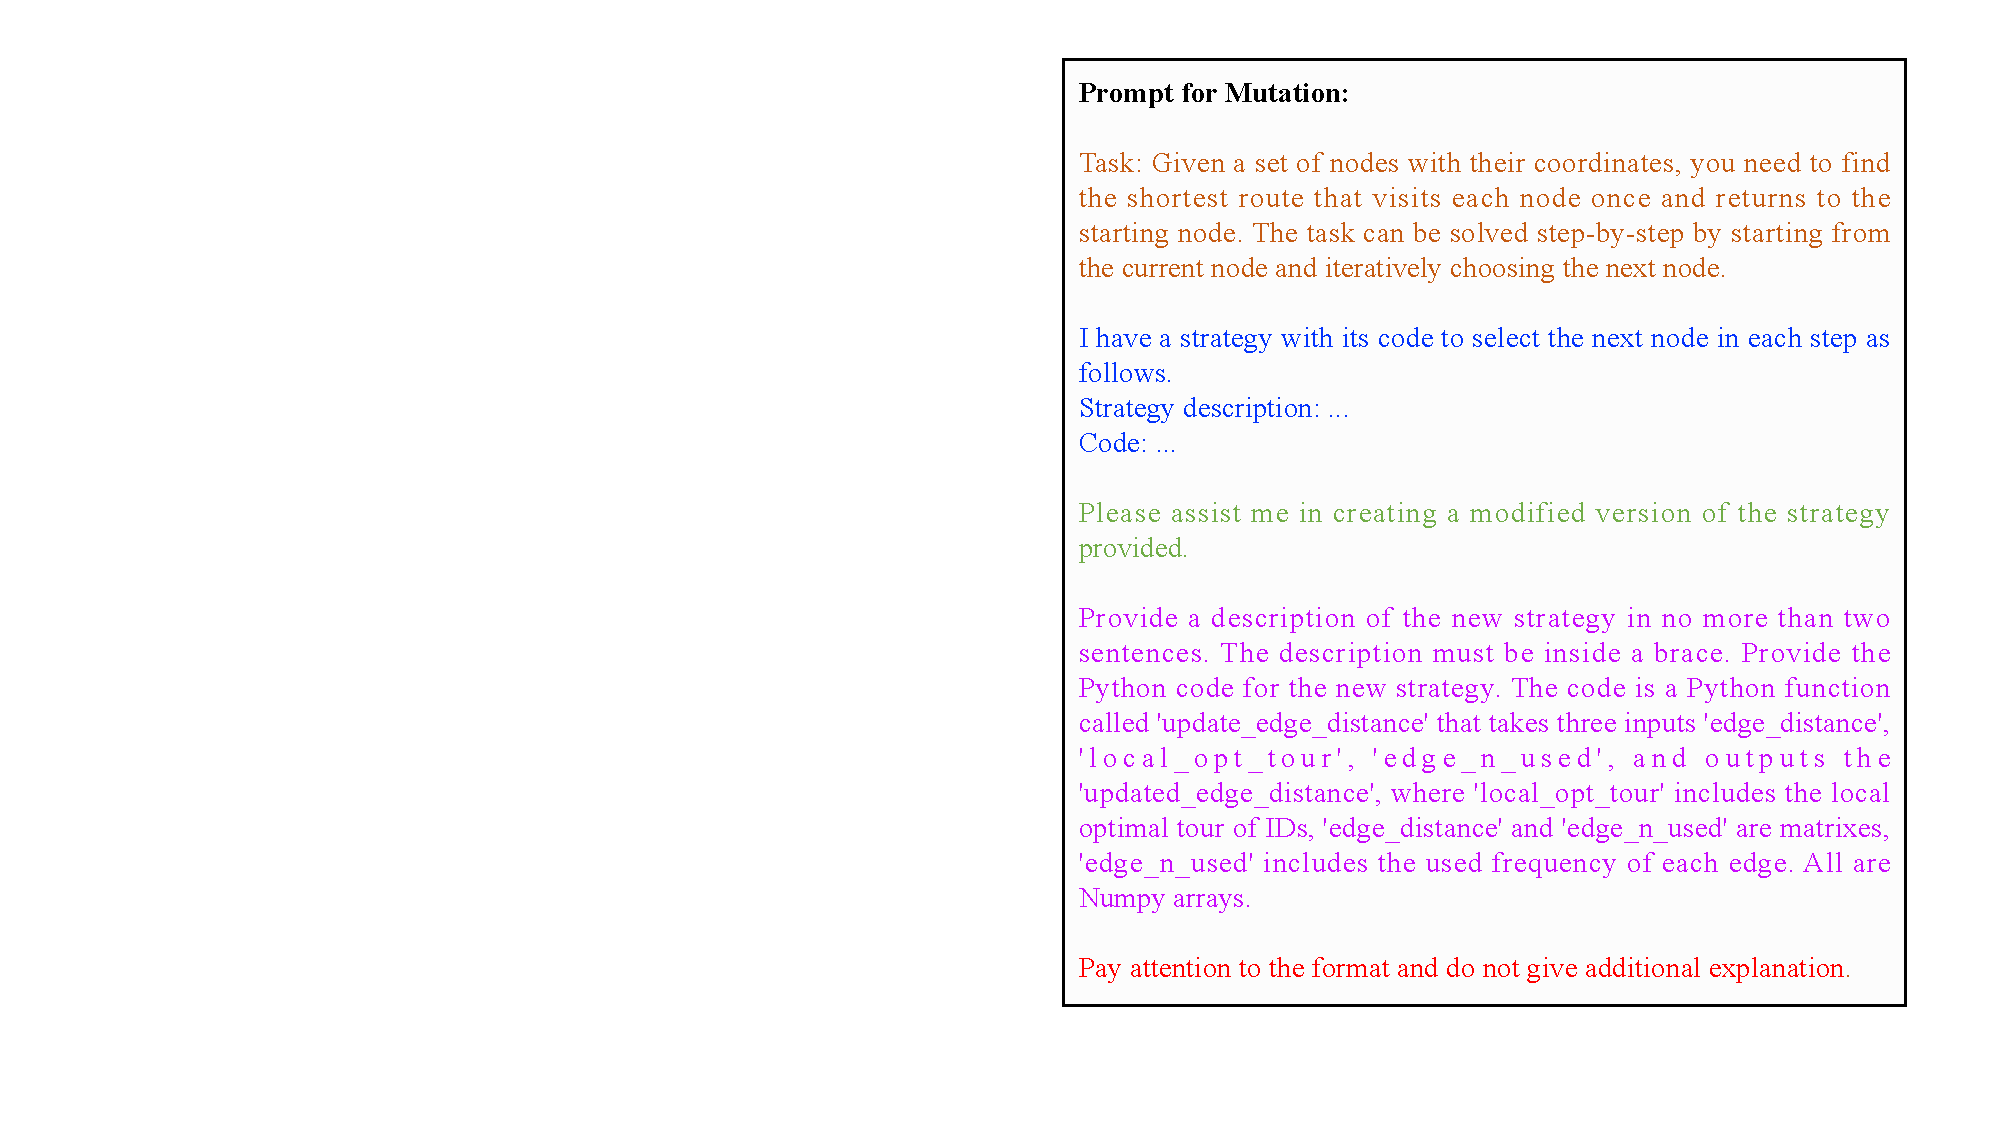
\includegraphics[width=\linewidth]{figures/Fig_mutation.pdf}
%         %\caption{}
%     \end{subfigure}
%     \caption{Prompts used in the initialization, crossover, and mutation of \ourmethod{} for TSP: \textcolor{brown}{A description of the task}, \textcolor{blue}{Parent heuristic(s)}, \textcolor{darkgreen}{Prompt-specific hints}, \textcolor{purple}{An expected output}, and \textcolor{red}{Other hints}.}
%     \label{fig:prompt}
% \end{figure}

\subsection{Designed Heuristic Strategy}

Figure~\ref{fig:heuristic_tsp} illustrates the heuristic strategy designed by \ourmethod{} for updating the distance matrix for TSP. This matrix is obtained by modifying the original distance matrix and adding some random factors, which involves several intermediate variables, including the average of distances, the average of edge used, and a penalty on the current local optimal route.

\begin{figure}[ht]
\caption{Heuristic strategy designed by \ourmethod{} on TSP. }~\label{fig:heuristic_tsp}

\begin{minipage}{0.99\linewidth}
\begin{lstlisting}

|\textbf{Heuristic Designed by \textcolor{red}{\ourmethod{}}}|

|\textbf{<Heuristic Description>}|
|\text{Update the edge distances in the edge distance matrix by }|
|\text{incorporating a pheromone-like effect, where the update is determined by edge count, }|
|\text{distance, and usage, with the addition of a decay factor to }|
|\text{avoid stagnation and promote exploration. }|

|\textbf{<Code>}|
import numpy as np

def heuristic(edge_distance, local_opt_tour, edge_n_used):
    updated_edge_distance = np.copy(edge_distance)
    edge_count = np.zeros_like(edge_distance)
    for i in range(len(local_opt_tour) - 1):
        start = local_opt_tour[i]
        end = local_opt_tour[i + 1]
        edge_count[start][end] += 1
        edge_count[end][start] += 1
        # penalize local optimal route
    edge_n_used_max = np.max(edge_n_used) 
        # calculate the average edge used
    decay_factor = 0.1 # decay fastor
    mean_distance = np.mean(edge_distance) 
        # calculate the average distance
    for i in range(edge_distance.shape[0]):
        for j in range(edge_distance.shape[1]):
            if edge_count[i][j] > 0:
                noise_factor = (np.random.uniform(0.7, 1.3) / edge_count[i][j]) + (edge_distance[i][j] / mean_distance) - (0.3 / edge_n_used_max) * edge_n_used[i][j]
                    # calculate a hybrid noise factor
                updated_edge_distance[i][j] += noise_factor * (1 + edge_count[i][j]) - decay_factor * updated_edge_distance[i][j]
                    # The new guiding edge distance matrix is calculated based on both a noise term and a decayed original distance matrix

    return updated_edge_distance
\end{lstlisting}
\end{minipage}
\end{figure}

\subsection{More Experimental Results}~\label{more_results_tsp}

We also compare the heuristic generated by EoH with the following methods: 
% Heuristics designed automatically by AI methods:
\begin{itemize}
    \item Graph Convolutional Network (GCN) method for TSP~\cite{joshi2019efficient}. 
    \item  Attention Model (AM)~\cite{kool2018attention}. It uses neural networks to learn heuristics for combinatorial optimization. 
    \item  POMO~\cite{kwon2020pomo}. It adopts AM ideas and achieves state-of-the-art results. 
    \item LEHD~\cite{luo2023neural}. It is a new variant of AM with a different heavy decoder structure and is trained using supervised learning. 
    \item GLS~\cite{voudouris1999guided}. It is the vanilla version of GLS for TSP.
    \item EBGLS~\cite{shi2018eb}. It extends the GLS by considering the big valley feature of the TSP. 
    \item KGLS~\cite{arnold2019knowledge}. It uses multiple features extracted from previous knowledge of routing problems.  
    \item GNNGLS~\cite{hudson2021graph} and  NeuralGLS~\cite{sui2023neuralgls}. They use deep learning models in GLS. 
\end{itemize}
We set the maximum number of calls of LS to be 1,000 for each GLS algorithm on every test instance. We use the source code of POMO~\cite{kwon2020pomo} , BQ~\cite{drakulic2023bq}, and LEHD~\cite{luo2023neural} in our experiments. The experimental results for GNNGLS~\citet{hudson2021graph}, NeuralGLS~\citet{sui2023neuralgls}, AM~\citet{hudson2021graph} and GCN ~\citet{sui2023neuralgls} are directly extracted from their respective papers. The solutions obtained by Concorde~\cite{applegate2006concorde} are used as the baselines for computing the performance gap. 

We consider three different numbers of locations: 20, 50, and 100. For each number of locations, we randomly generate 1,000 locations from $[0,1]^2$ and thus obtain 1,000 test instances.  
Table~\ref{table:tsprandom_appendix} shows the average performance of the heuristics on these random instances. The table provides the average gap compared with the baseline solver Concorde, as well as the average running time on each instance. It should be pointed out that POMO, BQ, and LEHD run in a parallel manner on the GPU, so single-instance running time is not provided. It is very clear from Table~\ref{table:tsprandom_appendix} that the heuristic produced by 
EoH performs the best.  

%While recent works like BQ and LEHD aim for cross-size generalization and have shown promising results on large-scale problems, they are trained using supervised learning on diverse-sized training data. not relevent. 

% Among the GLS varaints, KGLS performs the best with an average gap of 0.035\% on TSP100 instances. EoH-GLS can reduce this gap to 0.032\% on the TSP100 instances. Comparing EoH-GLS with GNNGLS and NeuralGLS, we observe a significant reduction in the average gap. Specifically, our approach achieves an impressive reduction from 0.47\% (as reported in NeuralGLS) to 0.032\%. Furthermore, our approach accomplishes this reduction in a considerably shorter running time. However, it is crucial to acknowledge that our results for GNNGLS and NeuralGLS are based on their respective papers, as the code for NeuralGLS is not publicly available. Additionally, differences in running environments and implementation methods need to be considered, as they may introduce potential biases in a direct comparison.


\begin{table}[tbp]
\centering
\caption{Results on TSP20, TSP50, and TSP100. The gap and time are averaged over 1,000 instances.}~\label{table:tsprandom_appendix}
\small
\resizebox{0.7\textwidth}{!}{%
\begin{tabular}{lcccccc}
\toprule
\multirow{2}{*}{Method}& \multicolumn{2}{c}{TSP20}   & \multicolumn{2}{c}{TSP50}   & \multicolumn{2}{c}{TSP100}   \\

& Gap (\%) & Time (s) & Gap (\%) & Time (s) & Gap (\%) & Time (s) \\
\midrule
 Concorde & 0.000    & 0.010    & 0.000    & 0.051    & 0.000    & 0.224    \\
 LKH3     & 0.000    & 0.020    & 0.000    & 0.069    & 0.011    & 0.118    \\
\midrule
NN  & 17.448   & 0.000    & 23.230   & 0.002    & 25.104   & 0.010    \\
 FI & 2.242    & 0.005    & 7.263    & 0.065    & 12.456   & 0.444    \\
 AM & 0.069    & 0.038    & 0.494    & 0.124    & 2.368    & 0.356    \\
 GCN& 0.035    & 0.974    & 0.884    & 3.080    & 1.880    & 6.127    \\
 POMO   & 0.120    & /  & 0.640    & /  & 1.070    & /  \\
 POMO aug8& 0.000    & /  & 0.030    & /  & 0.140    & /  \\
 BQ & 0.379    & /  & 0.245    & /  & 0.579    & /  \\
 LEHD     & 0.950    & /  & 0.485    & /  & 0.577    & /  \\
\midrule
 LS & 1.814    & 0.006    & 3.461    & 0.006    & 4.004    & 0.008    \\
GLS& 0.004    & 0.088    & 0.045    & 0.248    & 0.659    & 0.683    \\
 EBGLS    & 0.002    & 0.091    & 0.003    & 0.276    & 0.155    & 0.779    \\
 KGLS     & \textbf{0.000}    & 1.112    & \textbf{0.000}    & 3.215    & 0.035    & 7.468    \\
 GNNGLS & \textbf{0.000}    & 10.010   & 0.009    & 10.037   & 0.698    & 10.108   \\
 NeuralGLS & \textbf{0.000}    & 10.005   & 0.003    & 10.011   & 0.470    & 10.024   \\
\midrule
\ourmethod{}  & \textbf{0.000}    & 0.498    & \textbf{0.000}    & 1.494    & \textbf{0.025}    & 4.510   \\
\bottomrule
\end{tabular}%
}
\end{table}

We also conduct experiments on 29 TSPLib instances.
%, which were mostly derived from real-world problems and exhibited diverse geometric distributions. In our evaluation, we compared our \ourmethod{}-designed GLS  against various neural solvers such as AM, POMO, and LEHD, as well as different GLS algorithms including GNNGLS, NeuralGLS, LS, GLS, EBGLS, and KGLS. The results for AM, GNNGLS, and NeuralGLS were obtained from the respective papers \cite{hudson2021graph,sui2023neuralgls}, while the remaining algorithms were evaluated by us. We set the maximum number of iterations to 1,000 for each instance.
As shown in Table~\ref{table:TSPLibresults}, The GLS algorithm designed by \ourmethod{} outperforms all the other heuristics including hand-crafted ones in terms of the average gap on the 29 instances. 

% Notably, when compared with the neural solvers, the average gap significantly reduced from 1.91\% to 0.28\%. Furthermore, our results also surpassed all the GLS algorithms designed by human experts.

\begin{table*}[htbp]
\centering
\caption{Results on TSPLib instances. The gap (\%) to the best-known solution from TSPLib.}~\label{table:TSPLibresults}
\large
\renewcommand\arraystretch{0.95}
\resizebox{0.7\textwidth}{!}{%
\begin{tabular}{ccccccccccc}
\toprule
\multicolumn{1}{c}{\multirow{2}{*}{Instance}} & \multicolumn{3}{c}{Other Algorithms} & \multicolumn{6}{c}{GLS Algorithms} & \multirow{2}{*}{\ourmethod{}} \\
\multicolumn{1}{c}{}  & AM& POMO & LEHD& GNNGLS & NeuralGLS & LS    & GLS   & EBGLS & KGLS  &  \\
\midrule
eil51    & 1.63   & 0.83  & 1.64  & 0.00 & 0.00 & 2.85 & 0.67 & 0.67 & 0.67 & 0.67 \\
berlin52 & 4.17   & 0.04  & 0.03  & 0.14 & 0.00 & 3.89 & 0.03 & 0.03 & 0.03 & 0.03 \\
st70     & 1.74   & 0.31  & 0.33  & 0.76 & 0.00 & 2.64 & 0.31 & 0.31 & 0.31 & 0.31 \\
eil76    & 1.99   & 1.18  & 2.54  & 0.16 & 0.00 & 3.93 & 1.37 & 1.18 & 1.18 & 1.48 \\
pr76     & 0.82   & 0.00  & 0.22  & 0.04 & 0.82 & 6.71 & 0.00 & 0.00 & 0.00 & 0.00 \\
rat99    & 2.65   & 2.39  & 1.10  & 0.55 & 0.72 & 6.58 & 1.55 & 0.74 & 0.68 & 0.68 \\
kroA100  & 4.02   & 0.41  & 0.12  & 0.73 & 0.03 & 3.00 & 0.02 & 0.02 & 0.06 & 0.02 \\
kroB100  & 5.14   & 0.32  & 0.26  & 0.15 & 0.88 & 0.58 & 0.23 & 0.00 & 0.25 & 0.00 \\
kroC100  & 0.97   & 0.18  & 0.32  & 1.57 & 1.77 & 4.70 & 0.50 & 0.01 & 0.01 & 0.01 \\
kroD100  & 2.72   & 0.84  & 0.38  & 0.57 & 0.00 & 5.67 & 0.00 & 0.20 & 0.00 & 0.00 \\
kroE100  & 1.47   & 0.45  & 0.43  & 1.22 & 1.05 & 4.64 & 0.49 & 0.00 & 0.07 & 0.14 \\
rd100    & 3.41   & 0.01  & 0.01  & 0.46 & 0.00 & 1.27 & 0.01 & 0.01 & 0.02 & 0.01 \\
eil101   & 2.99   & 1.84  & 2.31  & 0.20 & 0.36 & 8.82 & 3.28 & 1.91 & 2.07 & 2.27 \\
lin105   & 1.74   & 0.52  & 0.34  & 0.61 & 0.65 & 1.87 & 0.03 & 0.03 & 0.03 & 0.03 \\
pr107    & 3.93   & 0.52  & 11.24 & 0.44 & 0.81 & 0.72 & 0.40 & 0.00 & 0.00 & 0.00 \\
pr124    & 3.68   & 0.60  & 1.11  & 0.76 & 0.08 & 2.44 & 0.60 & 0.60 & 0.08 & 0.00 \\
bier127  & 5.91   & 13.72 & 4.76  & 1.95 & 2.73 & 1.79 & 0.59 & 0.29 & 0.42 & 0.42 \\
ch130    & 3.18   & 0.16  & 0.55  & 3.52 & 1.19 & 7.61 & 1.09 & 0.46 & 0.01 & 0.01 \\
pr136    & 5.06   & 0.93  & 0.45  & 3.39 & 2.32 & 6.30 & 2.01 & 0.28 & 0.24 & 0.00 \\
pr144    & 7.64   & 0.53  & 0.19  & 3.58 & 0.74 & 4.19 & 0.09 & 0.00 & 0.00 & 0.00 \\
ch150    & 4.58   & 0.53  & 0.52  & 2.11 & 2.49 & 1.35 & 0.68 & 0.37 & 0.04 & 0.24 \\
kroA150  & 3.78   & 0.70  & 1.40  & 2.98 & 0.77 & 5.05 & 1.75 & 0.26 & 0.17 & 0.00 \\
kroB150  & 2.44   & 1.17  & 0.76  & 3.26 & 3.11 & 5.55 & 1.01 & 0.00 & 0.08 & 0.00 \\
pr152    & 7.49   & 1.05  & 12.14 & 3.12 & 0.00 & 2.75 & 0.19 & 0.19 & 0.19 & 0.19 \\
u159     & 7.55   & 0.95  & 1.13  & 1.02 & 0.90 & 5.63 & 0.74 & 0.78 & 0.96 & 0.00 \\
rat195   & 6.89   & 8.15  & 1.42  & 1.67 & 0.48 & 2.14 & 0.61 & 0.61 & 0.97 & 0.82 \\
d198     & 373.02 & 17.29 & 9.23  & 4.77 & 1.28 & 7.96 & 2.08 & 1.87 & 0.31 & 0.59 \\
kroA200  & 7.11   & 1.58  & 0.64  & 2.03 & 0.86 & 0.91 & 0.75 & 0.18 & 0.71 & 0.15 \\
kroB200  & 8.54   & 1.44  & 0.16  & 2.59 & 3.74 & 4.71 & 1.43 & 1.27 & 0.89 & 0.20 \\
\midrule
Average  & 16.77  & 2.02  & 1.92  & 1.53 & 0.96 & 4.01 & 0.78 & 0.42 & 0.36 & 0.28 \\
\bottomrule
\end{tabular}%
}
\end{table*}



\section{Flow Shop Scheduling Problem}


\subsection{Prompt Engineering}

This subsection is to introduce details of prompt engineering used for FSSP. We use the same components for bin packing. Figure~\ref{fig:prompt_fssp} provides two illustrative examples of prompts for initialization and E2, with each component represented in a different color. 

\begin{figure}[t]
    \centering
    \caption{Two examples of prompt engineering used in initialization and E2 strategy for FSSP.}
    \label{fig:prompt_fssp}

\begin{minipage}{0.38\textwidth}
\small
\begin{dialogbox}
  \textbf{Prompt for Initialization} \\
  
  \textcolor {darkbrown}{I have n jobs and m machines. Help me create a new heuristic to update the execution time matrix and select the top jobs to perturb to avoid being trapped in the local optimum scheduling with the final goal of finding scheduling with minimized makespan.} \\

  Please design a new heuristic.
  
  \textbf{Firstly,} describe your \textcolor{navyblue}{new heuristic and main steps in one sentence}. \\
  \textbf{Next,} implement it in Python as a function named \textcolor{navyblue}{'get\_matrix\_and\_jobs'}. This function should accept \textcolor{navyblue}{four inputs: "current\_sequence","time\_matrix","m","n"}. The function should return \textcolor{navyblue}{two output: "new\_matrix",'perturb\_jobs'}. \textcolor{navyblue}{The variable 'current\_sequence' represents the current sequence of jobs. The variables 'm' and 'n' denote the number of machines and number of jobs, respectively. The variable 'time\_matrix' is a matrix of size n*m that contains the execution time of each job on each machine. The output 'new\_matrix' is the updated time matrix, and 'perturb\_jobs' includes the top jobs to be perturbed.}  \\

  \textcolor{purple}{The matrix and job list are Numpy arrays. Do not give additional explanations.}
\end{dialogbox}
\end{minipage}
\begin{minipage}{0.61\textwidth}
\small
\begin{dialogbox}
  \textbf{Prompt for E2} \\
  
  \textcolor[HTML]{8B4513}{I have n jobs and m machines. Help me create a new heuristic to update the execution time matrix and select the top jobs to perturb to avoid being trapped in the local optimum scheduling with the final goal of finding scheduling with minimized makespan.} \\

  \textcolor{darkgreen}{I have five existing heuristics with their codes as follows: \\
  No.1 Heuristic description: \\
       Code:   \\
       ... \\
  No.5 Heuristic description: \\
       Code: \\  } 
       
   Please help me design a new heuristic that is different from the given ones but can be motivated by them. \\
   \textbf{Firstly,} identify the common idea in the provided heuristics.   \\
   \textbf{Secondly,} based on the backbone idea \textcolor{navyblue}{describe your new heuristic in one sentence.} \\
   \textbf{Thirdly,} implement it in Python as a function named \textcolor{navyblue}{'get\_matrix\_and\_jobs'}. This function should accept \textcolor{navyblue}{four inputs: "current\_sequence","time\_matrix","m","n"}. The function should return \textcolor{navyblue}{two output: "new\_matrix",'perturb\_jobs'}. \textcolor{navyblue}{The variable 'current\_sequence' represents the current sequence of jobs. The variables 'm' and 'n' denote the number of machines and number of jobs, respectively. The variable 'time\_matrix' is a matrix of size n*m that contains the execution time of each job on each machine. The output 'new\_matrix' is the updated time matrix, and 'perturb\_jobs' includes the top jobs to be perturbed.}   \\

  \textcolor{purple}{The matrix and job list are Numpy arrays. Do not give additional explanations.}
\end{dialogbox}
\end{minipage}
\end{figure}


\subsection{Designed Heuristic Strategy}
We adopt the same GLS framework with two selected local search operators: Swap and Relocate. EoH is used to design a heuristic strategy for updating both the execution time matrix and to determine the perturbed jobs. 
%The perturbation is performed to a list of jobs and  in the perturb job list on the updated execution time matrix. 
Figure~\ref{fig:heuristic_fssp} illustrates a heuristic designed by \ourmethod{} for FSSP. Some selected elements in the original matrix are updated. 
%Figure~\ref{fig:heuristic_fssp} illustrates the heuristic designed by \ourmethod{} for FSSP. A subset of the original matrix is randomly selected. The subset is updated with a perturbation factor to form an updated matrix. 


\begin{figure}[ht]
\caption{Heuristic strategy designed by \ourmethod{} on FSSP. }~\label{fig:heuristic_fssp}

\begin{minipage}{0.99\linewidth}
\begin{lstlisting}

|\textbf{Heuristic Designed by \textcolor{red}{\ourmethod{}}}|

|\textbf{<Heuristic Description>}|
|\text{The heuristic randomly selects a subset of machines, computes the weighted }|
|\text{average execution time  for each job on the selected machines, }|
|\text{and perturbs the top jobs in the current sequence to update the }|
|\text{execution time matrix by scaling the original execution time with }|
|\text{a random perturbation factor between 0.8 and 1.2.}|


|\textbf{<Code>}|
import numpy as np
def heuristic(current_sequence, time_matrix, m, n):
    machine_subset = np.random.choice(m, max(1, int(0.3*m)), replace=False)
        # randomly select a subset of machines
    weighted_avg_execution_time = np.average(time_matrix[:, machine_subset], axis=1, weights=np.random.rand(len(machine_subset)))
        # compute the weighted average execution time
    perturb_jobs = np.argsort(weighted_avg_execution_time)[-int(0.3*n):]
        # sort the last jobs based on the weighted average execution time
    new_matrix = time_matrix.copy()
    perturbation_factors = np.random.uniform(0.8, 1.2, size=(len(perturb_jobs), len(machine_subset)))
        # calculate perturbation factors, introduce certain randomness
    new_matrix[perturb_jobs[:, np.newaxis], machine_subset] *= perturbation_factors
        # calculate the final guiding matrix
    return new_matrix, perturb_jobs
\end{lstlisting}
\end{minipage}
\end{figure}



\subsection{More Results}~\label{more_results_fssp}
We also compare the heuristic produced by EoH with the following methods. 
\begin{itemize}
\item GUPTA~\cite{gupta1971functional}. It is a classic heuristic algorithm for FSSP.
\item CDS~\cite{campbell1970heuristic}. It is a classic heuristic algorithm for FSSP.
\item  NEH~\cite{nawaz1983heuristic}. It is widely recognized as an efficient heuristic for FSSP.
\item NEHFF~\cite{fernandez2014insertion}. It is a revision of NEH.
\item PFSPNet and PFSPNet\_NEH~\cite{pan2021deep}. They are recently developed deep learning solvers for flow-shop scheduling.
\item Local Search (LS). It is the basic local search with the same operators used in EoH. 
\item ILS1~\cite{stutzle1998applying}: It is an iterated local search developed for FSSP.
\item ILS2: It uses the same framework as ours but with hand-crafted heuristic strategy.
%which has shown promising results in flow-shop scheduling. Moreover, we implemented the revised iterated local search algorithm~\cite{lourencco2019iterated}, using the exact same framework as our own (referred to as ILS2).
\end{itemize}


% investigated heuristics based on local search. We started with the basic local search approach without any guidance or perturbation (referred to as LS). Additionally, we examined the iterated local search proposed by ILS1~\cite{stutzle1998applying}, which has shown promising results in flow-shop scheduling. Moreover, we implemented the revised iterated local search algorithm~\cite{lourencco2019iterated}, using the exact same framework as our own (referred to as ILS2).

We evaluate the algorithms on the widely-used Taillard Instances. We test 11 different test sets.  The number of jobs in these instances ranges from 20 to 200, and the number of machines ranges from 5 to 20.


Table~\ref{table:taillard_appendix} presents the results obtained from different algorithms on Taillard instances. The table gives the average gaps to the upper bounds provided in~\citet{taillard1993benchmarks}. The average is calculated on 10 instances for each test set. The best results are highlighted in bold. \ourmethod{} is the best on most test sets and obtain the best average gap of 0.23\%. \ourmethod{} outperforms these commonly used heuristics as well as the recent deep learning neural solvers. Notably, \ourmethod{} outperforms ILS2, which shares the same framework and local search operators but uses a human hand-crafted heuristic strategy for perturbation.


\begin{table}[t]
\centering
\caption{Results on Taillard instance sets. The value is the average gap to the best-known solutions on 10 instances in each set. The best results are in bold. }~\label{table:taillard_appendix}

\resizebox{0.7\textwidth}{!}{%
\begin{tabular}{lccccccccc}
\toprule

  Test Set& GUPTA & CDS   & NEH  & NEHFF & PFSPNet & LS   & ILS1 & ILS2  & \ourmethod{}    \\
\midrule
20\_5   & 12.89 & 9.03  & 3.24 & 2.30  & 2.30 & 1.91 & 0.42 & 0.18  & \textbf{0.09}  \\
20\_10  & 23.42 & 12.87 & 4.05 & 4.15  & 4.04 & 2.77 & 0.33 & \textbf{0.25} & \textbf{0.30}  \\
20\_20  & 21.79 & 10.35 & 3.06 & 2.72  & 2.96 & 2.60 & 0.29 & 0.25  & \textbf{0.10}  \\
\midrule
50\_5   & 12.23 & 6.98  & 0.57 & 0.40  & 0.51 & 0.32 & 0.15 & 0.32  & \textbf{0.02}  \\
50\_10  & 20.11 & 12.72 & 3.47 & 3.62  & 3.48 & 3.33 & 1.47 & 0.29  & \textbf{0.19}  \\
50\_20  & 22.78 & 15.03 & 5.48 & 5.10  & 5.05 & 4.67 & 2.13 & \textbf{0.34} & 0.60   \\
\midrule
100\_5  & 5.98  & 5.10  & 0.39 & 0.31  & 0.31 & 0.28 & 0.20 & 0.38  & \textbf{-0.04} \\
100\_10 & 15.03 & 9.36  & 2.07 & 1.88  & 1.72 & 1.38 & 0.77 & 0.34  & \textbf{0.14}  \\
100\_20 & 21.00 & 13.55 & 3.58 & 3.73  & 3.56 & 3.51 & 2.27 & \textbf{0.43} & \textbf{0.41}  \\
200\_10 & 11.59 & 7.22  & 0.98 & 0.70  & 0.82 & 0.87 & 0.74 & 0.54  & \textbf{0.12}  \\
\midrule
200\_20 & 18.09 & 11.89 & 2.90 & 2.52  & 2.49 & 2.53 & 2.26 & \textbf{0.59} & \textbf{0.61}  \\
\midrule
Average & 16.81 & 10.37 & 2.71 & 2.49  & 2.48 & 2.20 & 1.00 & 0.36  & \textbf{0.23} \\
\bottomrule
\end{tabular}%
}
\end{table}


